\section{Analysis}
This chapter describes the first step of this project, the research of published technical reports and tools which are considered interesting for this project. The individual sections are again divided into a short description and a conclusion of how valuable this will be for the project. In the case of tested tools, the difficulties during the tests are also discussed.
\subsection{BloodHound / SharpHound}
\subsubsection{Description}
%Lukas
BloodHound describes itself on its wiki page on GitHub as follows:
\begin{quotation}
    \textit{''BloodHound is a single page Javascript web application, built on top of Linkurious, compiled with Electron, with a Neo4j database fed by a PowerShell/C\# ingestor. BloodHound uses graph theory to reveal the hidden and often unintended relationships within an Active Directory environment. Attacks can use BloodHound to easily identify highly complex attack paths that would otherwise be impossible to quickly identify. Defenders can use BloodHound to identify and eliminate those same attack paths. Both blue and red teams can use BloodHound to easily gain a deeper understanding of privilege relationships in an Active Directory environment.'' \cite{blo2018}} 
\end{quotation}
\subsubsection{Difficulties}
BloodHound was tested in the test environment which is described later in this chapter. Both the C\# and Python ingestors were successfully installed and tested. The only problem which occurred was that the Python-ingestor does not yet run on the latest Python release. One must have a Python 2.7.x version installed to run the scripts successfully.

\subsubsection{Conclusion}
The most interesting aspect of BloodHound for our project is the way it retrieves its data. Due to the decision that the application, in a first step, only reads the data of the local computer and not the whole domain, BloodHound will only be important in a later part of the project. Their so called ingestor will be used to retrieve the data of a whole network instead of only a local computer.

\subsection{Windows Event Logging Forensic Logging Enhancement Services}
\subsubsection{Description}
Windows Event Logging Forensic Logging Enhancement Services (WEFFLES) is a Threat Hunting/Incident Response Console with Windows Event Forwarding and PowerBI, coded and published by Microsoft-Security-Employee Jessica Payne. It is built to help set up the Windows Event Forwarding, so that all the collected logs of a system are stored on one centralised server, and afterwards to analyse the collected data. Jessica Payne wrote an installation instruction on the Microsoft TechNet blog \url{https://blogs.technet.microsoft.com/jepayne/2017/12/08/weffles/}. Once the data is collected  the generated weffels.csv file can simply be imported into Excel and start filtering the logs to gain the needed. Jessica Payne recommends to use PowerBI, a business analytics tool designed by Microsoft. In her published blog she also gives a short introduction on what to look out for, which event ids are important and other useful tips and tricks for detecting suspicious activities in the network.
\subsubsection{Conclusion}
WEFFELS will not be the product on which this project is based, but could become an important point of reference. The installation guide and other WEFFELS-related documents collected by Jessica Payne provide a lot of information for reading and understanding logs, which will be very helpful for this project. Also an interesting aspect of WEFFLES and the Jessica Payne article is how she visualised the logs, using Microsoft PowerBI.


\subsection{Microsoft Security Compliance Toolkit}
\subsubsection{Description}
The Microsoft Security Compliance Toolkit (SCT) \cite{SCT} allows security administrators to analyse their configured enterprise Group Policy Objects (GPO) in comparison to the Microsoft-recommended GPO baselines. The toolkit comes with  several baseline GPO's for different versions of Microsoft Windows Client and Servers:
% handed with -> comes with or is delivered with

\begin{itemize}
    \item Windows 10 security baselines
    \begin{itemize}
        \item Windows 10 Version 1803 (April 2018 Update), 1709 (Fall Creators Update), 1703 (Creators Update), 1607 (Anniversary Update), 1511 (November Update), 1507
    \end{itemize}
    \item Windows Server security baselines
    \begin{itemize}
        \item Windows Server 2016
        \item Windows Server 2012 R2
    \end{itemize}
    \item Microsoft Office security baseline
    \begin{itemize}
        \item Office 2016
    \end{itemize}
\end{itemize}

\subsubsection{Difficulties}
The toolkit is very simple and could be understood and used without any difficulties. The handling is very intuitive and does not require much training. Please note, however, that the toolkit cannot be used with Windows 10 Home, since active directory support is not provided with this version.

\subsubsection{Conclusion}
This toolkit can be used for a very baseline GPO in enterprise environment. With the delivered baselines it is easy to compare the configured GPO and to see the readiness of the enterprise GPO. The toolkit enables the comparison of different local GPO's installed on different Clients or Servers to check their consistency. In addition, the provided baselines can be used for building new GPO's. Furthermore, Microsoft delivers with the SCT a Local Group Policy Object Utility (LGPO.exe) to:
\begin{itemize}
    \item Import and apply policy settings
    \item Export local policy to a GPO backup
    \item Parse a registry.pol file to "LGPO text" format
    \item Build a registry.pol file from "LGPO text"
\end{itemize}
This toolkit is very interesting, but cannot be used to build on it. The reason for this is that the source code of the complete toolkit is not available. However, it can be used as additional help for checking the readiness of a system and comparing the local policies against templates or other local policies.

\subsection{LogonTracer}
\subsubsection{Description}
JPCERT/CCs LogonTracer is a tool built to investigate malicious logons on a system based on the research described in section ''\ref{DetectingLateral} \nameref{DetectingLateral}''. The tool links hostnames or Internet-Protocol (IP) addresses with the \textit{"[...] account name found in logon-related events and displays it as a graph". \cite{LogonTracer}}  The following event ids are checked with the tool: 
\ \\
\begin{multicols}{2}
    \begin{itemize}
        \item 4624: Successful logon
        \item 4625: Logon failure
        \item 4768: Kerberos Authentication
        \item 4769: Kerberos Service Ticket
        \item 4776: NTLM Authentication
        \item 4672: Assign special privileges
    \end{itemize}
\end{multicols} \ \\
The following figure depicts a sample graph of logins from different users in the test environment:
\begin{figure}[H]
    \centering
    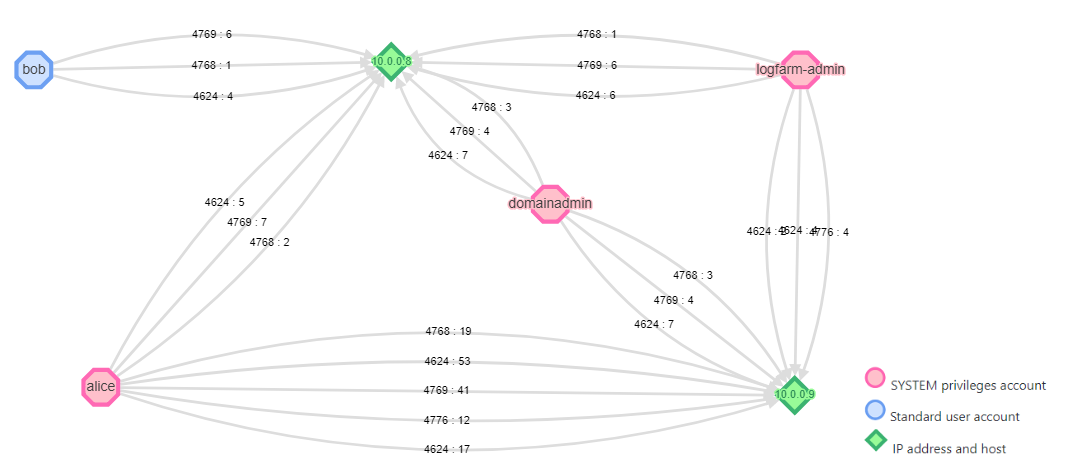
\includegraphics[width=0.8\linewidth]{assets/LogonTracer/LogonTrace_LogFarm.png}
    \caption{LogonTracer: Sample Graph from Test Environment}
    \label{fig:LogonTracerSample}
\end{figure}
\ \\
To use the LogonTracer, only a .evtx-File (Windows Extensible Markup Language (XML) Event Log: export of Windows event logs) is necessary to be uploaded. To get the best result out of LogonTracer an export of the security event log from the domain controller should be used - to get as much information of the network as possible. With the built-in analysis of logins, by using machine learning models and statistical analysis, LogonTracer is able to provide a ranking of the most malicious users which tried to log in. \cite{LogonTracerBlog}
\\\\
In addition, LogonTracer provides a timeline for all or selected users to show when each user logged in. The timeline can also be displayed as a graph with the LogonTracer, allowing anomalies to be detected more quickly.

\clearpage

The test environment showed that this graph can quickly become confusing - especially in a larger corporate environment as depicted in figure \ref{fig:LogonTraceerConfusing} \nameref{fig:LogonTraceerConfusing}. Although only a small environment as described in the section \ref{sec:testenvironment} ''\nameref{sec:testenvironment}'' was used, it turned out that various users wanted to log on to the virtual machines. The reason for this is that the test environment was built in the Microsoft Azure Cloud and is accessible via public IP addresses in the cloud.

\begin{figure}[H]
    \centering
    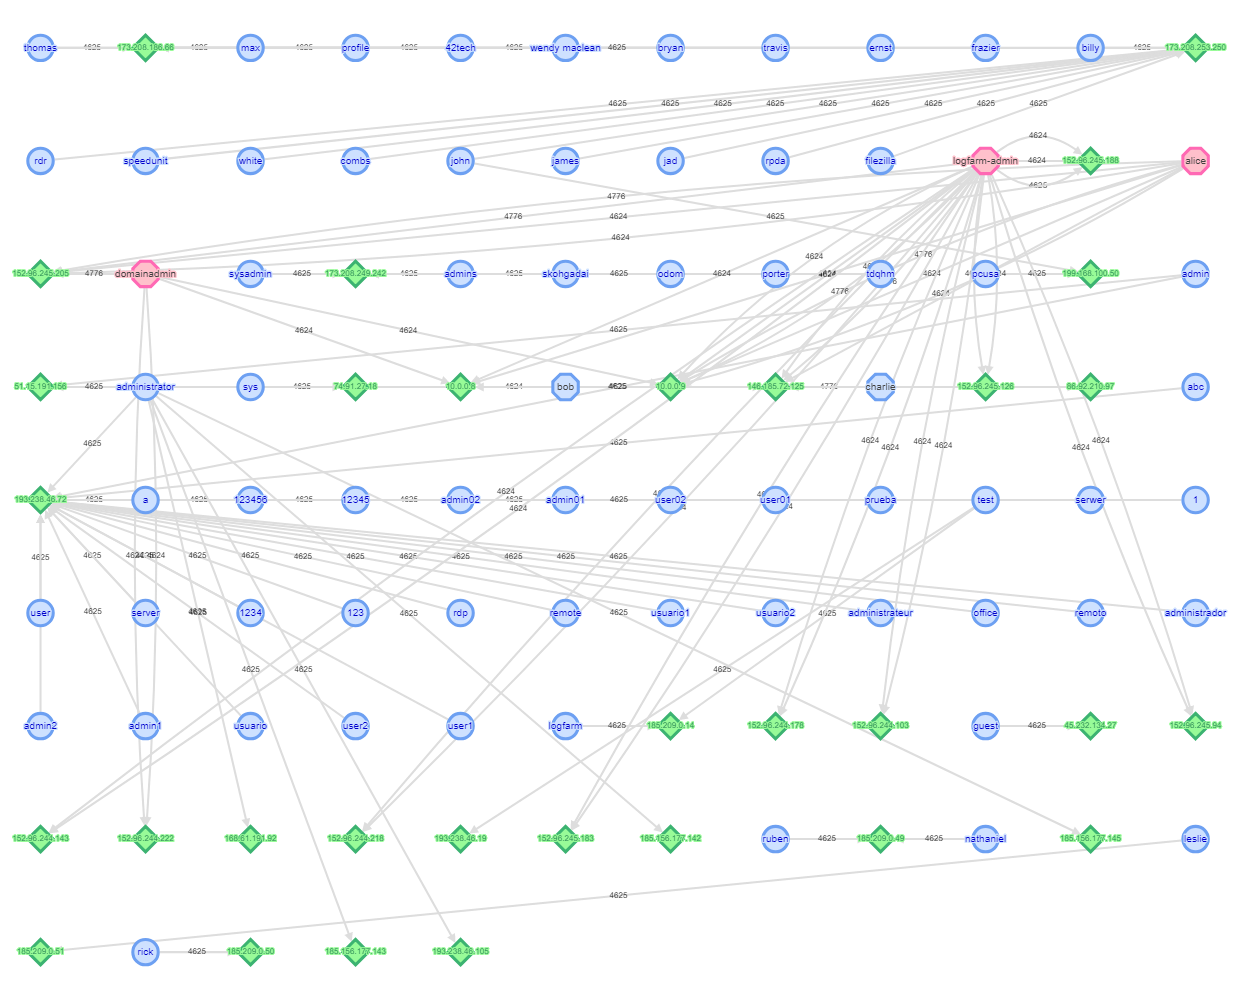
\includegraphics[width=0.8\linewidth]{assets/LogonTracer/logontracer_confusing.png}
    \caption{LogonTracer: Confusing Graph from Test Environment}
    \label{fig:LogonTraceerConfusing}
\end{figure}

Nevertheless, with meaningful filters the search can be restricted and the graph can be used efficiently, as shown in figure \ref{fig:LogonTracerSample} \nameref{fig:LogonTracerSample}

\clearpage

\subsubsection{Difficulties}
During the test phase of LogonTracer some difficulties were faced. It is pretty easy to get the docker container, but starting LogonTracer was a bit of a challenge. JPCERT/CC gives the following instructions for starting the docker container:
\begin{lstlisting}[language=HTML,caption=LogonTracer: given docker run command]
    $ docker run --detach \
    --publish=7474:7474 --publish=7687:7687 --publish=8080:8080 \
    -e LTHOSTNAME=[IP_Address] jpcertcc/docker-logontracer
\end{lstlisting}
The problem was that the parameter \lstinline|[IP_Address]| was not described well. If the command \lstinline|docker ps| was executed it always showed the following \lstinline|PORTS|:
\begin{lstlisting}[caption=LogonTracer: docker ps (PORTS)]
    PORTS
    0.0.0.0:7474->7474/tcp, 0.0.0.0:7687->7687/tcp, 7473/tcp, 0.0.0.0:8080->8080/tcp
\end{lstlisting}
After some time of investigation and further tests, it turned out that under \lstinline|PORTS| the ports respectively ip addresses of the container can be bound to the host. But these are not relevant for the LogonTracer, because it provides a web application under the defined parameter \lstinline|[IP_Address]| and it can eventually be reached via \lstinline|localhost:8080|. If this parameter was set to \lstinline|127.0.0.1|, the database containing the imported .evtx file could not be accessed. Thus the graph was never displayed. The parameter \lstinline|[IP_Address]| set to \lstinline|localhost| solved this problem.

\begin{lstlisting}[language=HTML,caption=LogonTracer: recommended docker run command]
    $ docker run --detach \
    --publish=7474:7474 --publish=7687:7687 --publish=8080:8080 \
    -e LTHOSTNAME=localhost jpcertcc/docker-logontracer
\end{lstlisting}
\subsubsection{Conclussion}
The LogonTracer is unique in its form and should not be underestimated for the detection of lateral movements. This is because user access to various components available in the network can be visualised simply and graphically, hence conclusions can be drawn about what has happened.
\\\\
However, the LogonTracer is not suitable for detection readiness and cannot be used to build on it. Nonetheless, approaches for reading the event log for further work could be used. This tool is also extremely interesting and recommendable for a further detection of lateral movements.

\clearpage

\subsection{Microsoft Monitoring Active Directory for Signs of Compromise}
\subsubsection{Description}
This article ''Microsoft Monitoring Active Directory for Signs of Compromise'' \cite{MSADSignsOfCompromise} is about configuration of a solid event log monitoring for Microsoft servers. The article gives a quite a good overview about the audit policy in Microsoft systems and what each policy stands for. The article gives information about the most important audit policies and how noisy (if a lot of data is produced by them) they are. This study does not go into the details of the audit policies in detail. Furthermore, the article describes how the policies can be read with powershell.
\\\\
In this article Microsoft compiles in Appendix L \cite{MSAppendixL} all important event ids which are necessary for a successful detection of APTs and lateral movements.

\subsubsection{Conclussion}
Due to the fact that audit policies are an important setting for solid event logging, this article and Appendix L will be a central part of the toolkit to be built. As a next step and part of this study, these event ids have to be correlated with the event ids found in the JPCERT/CC's study "Detecting Lateral Movement through Tracking Event Logs" \cite{JPCERTDetectingLateralMovement} to make a clear statement which event ids have to be logged.

\subsection{MITRE Adversarial Tactics, Techniques and Common Knowledge (ATT\&CK)}
\subsubsection{Description}
MITRE ATT\&CK introduces itself on its website as follows:
\begin{quotation}
    \textit{''MITRE ATT\&CK™ is a globally-accessible knowledge base of adversary tactics and techniques based on real-world observations. The ATT\&CK knowledge base is used as a foundation for the development of specific threat models and methodologies in the private sector, in government, and in the cybersecurity product and service community.'' \cite{MITRE}} 
\end{quotation}
The portal offers a variety of attacks and their patterns, which are currently known in different operating systems. MITRE ATT\&CK describes the attack in short words and then lists possibilities for detection and mitigation. The portal also describes various attack tools, their targets and effects on the system. In addition, the corresponding attacks are always cross-referenced. This is a great advantage for a quick search, especially when time is of the essence.

\subsubsection{Conclusion}
Although many attacks are described and how they can be detected and fended off, MITRE ATT\&CK is not quite suitable for our task. The readiness of a system to detect tailored attacks and lateral movements is only roughly described and would be associated with a time-consuming analysis in order to draw exact conclusions.

\clearpage

\subsection{Sysmon}
\subsubsection{Description}
\begin{quotation}
    \textit{System Monitor (Sysmon) is a Windows system service and device driver that, once installed on a system, remains resident across system reboots to monitor and log system activity to the Windows event log. It provides detailed information about process creations, network connections, and changes to file creation time.\cite{Sysmon}}
\end{quotation}
Sysmon logs several events on the system which are partly logged by default too. For example, the event ''A new process has been created'' with the identifier (ID) 4688 is logged by Sysmon with the ID 1 ''Process Creation''. The problem is that the default logged event with the ID 4688 logs only the executable file (EXE) name as well as the including path. But bad guys want to stay below the radar, so they might replace the original EXE a with malicious one and rename it like the original. Hence, there is no way to determine with the system based event log entry 4688 if the original EXE was executed. Sysmon eliminates exactly this gap by logging not only the name and path of the EXE but also the hash value of the EXE. Ergo Sysmon brings a big advantage to detect if a malicious EXE was executed or not. thereforee a reference hash value of the executed EXE is required to compare the hash values on its correctness. \cite{Sysmon1}

\subsubsection{Conclusion}
As mentioned in the description, Sysmon is an important tool to be enabled for solid detection of attacks. So Sysmon has to be detected if it is running or not to prepare an environment for a good readiness. In order to not create duplicated events, the events similar logged by default and Sysmon must be examined by their differences. Very likely Sysmon is the better choice.


\subsection{Sysmon Tools}
% https://github.com/nshalabi/SysmonTools
\subsubsection{Description}
Sysmon Tools \cite{SysmonTools} contains some useful functions to make better use of Sysmon. Among other things there are different views for the representation of the single entries which were recorded by Sysmon. A Process View is provided which can be used to examine a process in more detail. Related processes are taken into account and represented in a simple data-flow-like view, sorted by chronological order. With the Map View you can include geo-locate IP addresses during the import phase and Map View tries to geo-map the network destinations with ipstack \cite{ipstack}. The All Events View represents a full search by Sysmon and can be filtered and grouped accordingly. Furthermore, Sysmon Tools offers a Sysmon Shell, which can be used to create a customized XML configuration for Sysmon using a graphical user interface (GUI). Templates are also provided for further building.
\subsubsection{Conclusion}
This tool can also be a great help for detecting attacks and, with the Sysmon Shell, a robust configuration for Sysmon can be created. However, Sysmon Tool will have no basis for this project.

\clearpage

\subsection{sysmon-modular}
\subsubsection{Description}
With sysmon-modular \cite{sysmon-modular} a clean configuration of the Windows system service System Monitor (Sysmon), an xml-file which is loaded by Sysmon, is provided. Noisy process creations, which are made by legitimate programs, are suppressed as far as possible by Sysmon. The tool offers the possibility and it is expressly recommended by the developer to adapt the configuration to the respective organisation. Furthermore, sysmon-modular implements various attacks in MITRE ATT\&CK for detection with Sysmon. It offers the possibility to detect the attacks shown in the figure \ref{fig:sysmonmodular} with Sysmon.

\begin{figure}[H]
    \centering
    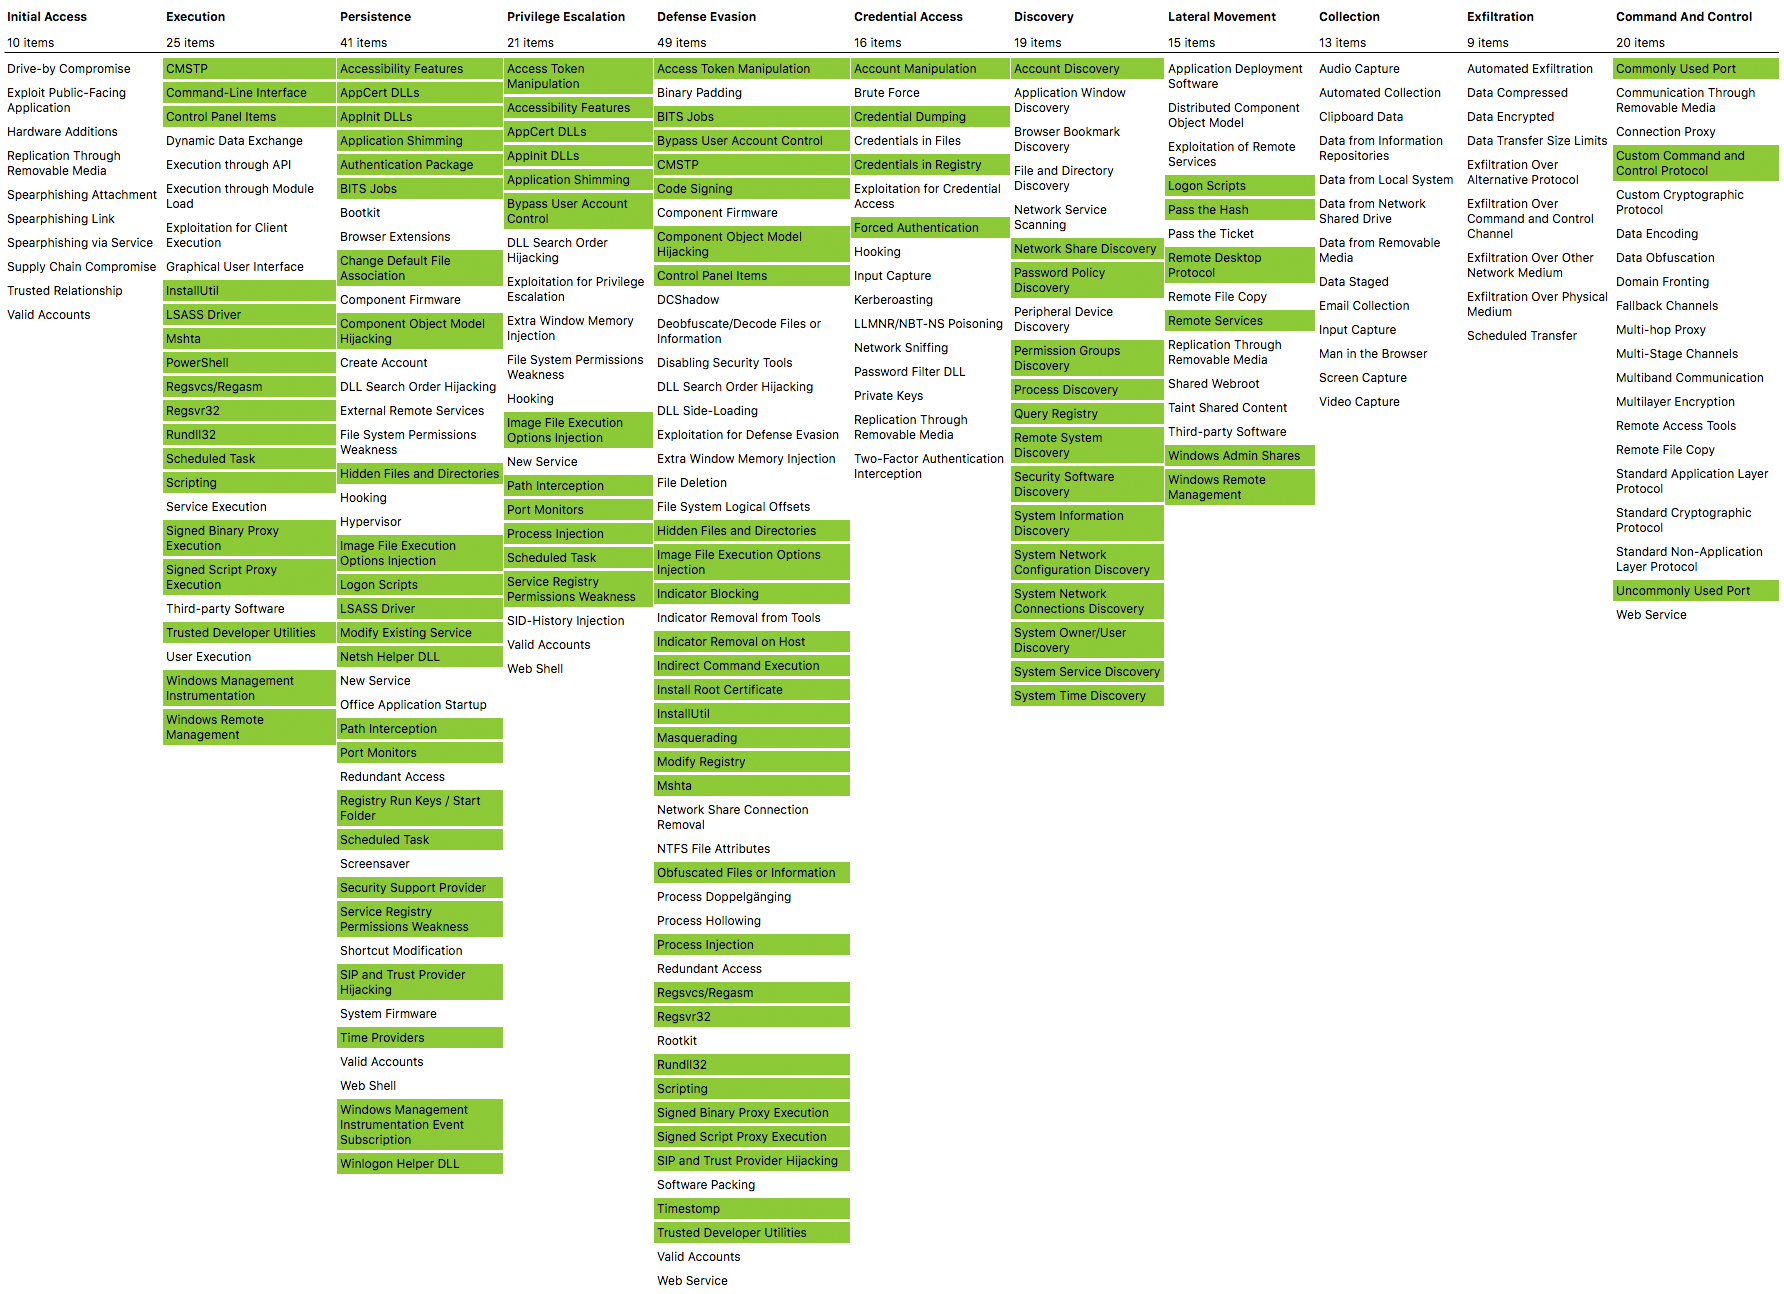
\includegraphics[width=1\linewidth]{assets/sysmon-modular/sysmon-modular.png}
    \caption{Detectable attacks with sysmon-modular}\label{fig:sysmonmodular}
\end{figure}

\subsubsection{Conclusion}
Sysmon-modular offers a very good basic configuration for Sysmon based on the platform MITRE ATT\&CK which is widely used in the security scene. Unfortunately, sysmon-modular was discovered when decisions were made to develop a tool based on the study "Detecting Lateral Movement through Tracking Event Logs" by JPCERT/CC. The readiness of a system with the basis of MITRE ATT\&CK patterns would probably have had an even greater impact. However, Sysmon-modular will most likely not be included in the tool during this study, unless there are still enough time reserves for such an integration. This tool would better fit the goal to realise a ''Readiness Optimizer'' as initially mentioned in the task definition.



\subsection{CryptoAPI 2.0} \label{CAPI2}
\subsubsection{Description}
The Microsoft feature CryptoAPI 2.0 (CAPI2) Diagnostics provides the ability to collect detailed information about certificate chain validation, certificate store operations and signature verification. CAPI2 in doubt extremely important for any Public Key Infrastructure (PKI) to perform several security based tasks, such as
\begin{itemize}
    \item Build and verify certificate chains
    \item Manage per-user and per-computer certificate stores
    \item Encrypt/decrypt, encode/decode and sign/verify messages
\end{itemize}
Hence, CAPI2 enables an organisation to secure its communications and business transactions. Identification of users, devices or organisation as well as signed e-mail, code signing and secure web browsing is made possible with today's standards of hash-functions and encryption due to CAPI2. PKI problems are not always easy to troubleshoot and therefore it is necessary to have good diagnostic capabilities in such cases. 
\begin{quotation}
    \textit{CAPI2 Diagnostics in Windows Vista\footnote{Windows Vista and above} provides logging of detailed information about certificate validation, network retrievals, revocation, and other low-level API results and errors. [...] utilizes the event logging and Event Viewer to provide better logging and troubleshooting capabilities for PKI applications based on the CAPI2 API set. \cite{CAPI2}}
\end{quotation}
\subsubsection{Conclusion}
To detect whether a system is ready for a good detection of lateral movements and APTs, CAPI2 is a core component to be logged in every system and CAPI2 Diagnostics must be enabled on a system. Hence, it is necessary to detect if CAPI2 is enabled on the system. On the other hand, CAPI2 Diagnostics produces a lot of events and therefore the log size should be chosen wisely. For this reason the recommendation of 4 Megabyte (MB) from Microsoft shall be applied. \cite{CAPI2}


\clearpage

\subsection{JPCERT/CC - Detecting Lateral Movement in APTs} \label{DetectingLateral}
\subsubsection{Description}
This document \cite{Abe2016} is from a presentation by Shingo Abe, a JPCERT/CC employee. In it he describes how to find system intruders more effectively using Windows Event Logs. The collected data is used to detect inconsistencies more effectively, such as when an administrator logs on to another machine or when an administrator logs on suspiciously often. 
\subsubsection{Conclusion}
This presentation contains interesting information which could be built into the project at a later point. The information this document contains is more suitable for monitoring purposes than for checking the readiness of a system.

\subsection{JPCERT/CC - Detecting Lateral Movement through Tracking Event Logs}\label{JPCertStudy}
\subsubsection{Description}
This is a document \cite{JPCERTDetectingLateralMovement} JPCERT/CC published in the year 2017. It describes how, in their experience, attackers proceed with lateral movement. In a very detailed 81-page report they describe the procedure step-by-step, the tools used and, what is most interesting for the project, the logs generated while doing so.
\subsubsection{Conclusion}
This report will have the biggest impact on this project, it shows which logs have to be read in any case. In addition, JPCERT/CC describes in this report which configurations are necessary for solid logging. The appendix not only describes the individual event log IDs, but also the audit policy that can be used to achieve them. For this reason, the checklist to be used will mainly be based on this report. With the provided information we see the greatest potential to develop a suitable tool for the accomplishment of the task in the given time. The given information of the configuration settings in JPCERT/CCs study appendix must be correlated with the ''Advanced security auditing Frequently Asked Questions (FAQ)'' \cite{AdvancedSecurityAuditing} in order to define the right auditing settings so that the right events are captured.

% \subsection{CAPI2}

